% Options for packages loaded elsewhere
\PassOptionsToPackage{unicode}{hyperref}
\PassOptionsToPackage{hyphens}{url}
%
\documentclass[
]{article}
\usepackage{lmodern}
\usepackage{amssymb,amsmath}
\usepackage{ifxetex,ifluatex}
\ifnum 0\ifxetex 1\fi\ifluatex 1\fi=0 % if pdftex
  \usepackage[T1]{fontenc}
  \usepackage[utf8]{inputenc}
  \usepackage{textcomp} % provide euro and other symbols
\else % if luatex or xetex
  \usepackage{unicode-math}
  \defaultfontfeatures{Scale=MatchLowercase}
  \defaultfontfeatures[\rmfamily]{Ligatures=TeX,Scale=1}
\fi
% Use upquote if available, for straight quotes in verbatim environments
\IfFileExists{upquote.sty}{\usepackage{upquote}}{}
\IfFileExists{microtype.sty}{% use microtype if available
  \usepackage[]{microtype}
  \UseMicrotypeSet[protrusion]{basicmath} % disable protrusion for tt fonts
}{}
\makeatletter
\@ifundefined{KOMAClassName}{% if non-KOMA class
  \IfFileExists{parskip.sty}{%
    \usepackage{parskip}
  }{% else
    \setlength{\parindent}{0pt}
    \setlength{\parskip}{6pt plus 2pt minus 1pt}}
}{% if KOMA class
  \KOMAoptions{parskip=half}}
\makeatother
\usepackage{xcolor}
\usepackage{tikz-network}


\definecolor{RosaMexicano}{RGB}{245, 0, 135}
\definecolor{Azul}{RGB}{0, 0, 255}
\definecolor{VerdeOlivo}{RGB}{172, 152, 60}
\definecolor{Verde}{RGB}{5, 135, 65}
\definecolor{Gris}{RGB}{170, 170, 170}
\IfFileExists{xurl.sty}{\usepackage{xurl}}{} % add URL line breaks if available
\IfFileExists{bookmark.sty}{\usepackage{bookmark}}{\usepackage{hyperref}}
\hypersetup{
  hidelinks,
  pdfcreator={LaTeX via pandoc}}
\urlstyle{same} % disable monospaced font for URLs
\usepackage{color}
\usepackage{fancyvrb}
\newcommand{\VerbBar}{|}
\newcommand{\VERB}{\Verb[commandchars=\\\{\}]}
\DefineVerbatimEnvironment{Highlighting}{Verbatim}{commandchars=\\\{\}}
% Add ',fontsize=\small' for more characters per line
\newenvironment{Shaded}{}{}
\newcommand{\AlertTok}[1]{\textcolor[rgb]{1.00,0.00,0.00}{\textbf{#1}}}
\newcommand{\AnnotationTok}[1]{\textcolor[rgb]{0.38,0.63,0.69}{\textbf{\textit{#1}}}}
\newcommand{\AttributeTok}[1]{\textcolor[rgb]{0.49,0.56,0.16}{#1}}
\newcommand{\BaseNTok}[1]{\textcolor[rgb]{0.25,0.63,0.44}{#1}}
\newcommand{\BuiltInTok}[1]{#1}
\newcommand{\CharTok}[1]{\textcolor[rgb]{0.25,0.44,0.63}{#1}}
\newcommand{\CommentTok}[1]{\textcolor[rgb]{0.38,0.63,0.69}{\textit{#1}}}
\newcommand{\CommentVarTok}[1]{\textcolor[rgb]{0.38,0.63,0.69}{\textbf{\textit{#1}}}}
\newcommand{\ConstantTok}[1]{\textcolor[rgb]{0.53,0.00,0.00}{#1}}
\newcommand{\ControlFlowTok}[1]{\textcolor[rgb]{0.00,0.44,0.13}{\textbf{#1}}}
\newcommand{\DataTypeTok}[1]{\textcolor[rgb]{0.56,0.13,0.00}{#1}}
\newcommand{\DecValTok}[1]{\textcolor[rgb]{0.25,0.63,0.44}{#1}}
\newcommand{\DocumentationTok}[1]{\textcolor[rgb]{0.73,0.13,0.13}{\textit{#1}}}
\newcommand{\ErrorTok}[1]{\textcolor[rgb]{1.00,0.00,0.00}{\textbf{#1}}}
\newcommand{\ExtensionTok}[1]{#1}
\newcommand{\FloatTok}[1]{\textcolor[rgb]{0.25,0.63,0.44}{#1}}
\newcommand{\FunctionTok}[1]{\textcolor[rgb]{0.02,0.16,0.49}{#1}}
\newcommand{\ImportTok}[1]{#1}
\newcommand{\InformationTok}[1]{\textcolor[rgb]{0.38,0.63,0.69}{\textbf{\textit{#1}}}}
\newcommand{\KeywordTok}[1]{\textcolor[rgb]{0.00,0.44,0.13}{\textbf{#1}}}
\newcommand{\NormalTok}[1]{#1}
\newcommand{\OperatorTok}[1]{\textcolor[rgb]{0.40,0.40,0.40}{#1}}
\newcommand{\OtherTok}[1]{\textcolor[rgb]{0.00,0.44,0.13}{#1}}
\newcommand{\PreprocessorTok}[1]{\textcolor[rgb]{0.74,0.48,0.00}{#1}}
\newcommand{\RegionMarkerTok}[1]{#1}
\newcommand{\SpecialCharTok}[1]{\textcolor[rgb]{0.25,0.44,0.63}{#1}}
\newcommand{\SpecialStringTok}[1]{\textcolor[rgb]{0.73,0.40,0.53}{#1}}
\newcommand{\StringTok}[1]{\textcolor[rgb]{0.25,0.44,0.63}{#1}}
\newcommand{\VariableTok}[1]{\textcolor[rgb]{0.10,0.09,0.49}{#1}}
\newcommand{\VerbatimStringTok}[1]{\textcolor[rgb]{0.25,0.44,0.63}{#1}}
\newcommand{\WarningTok}[1]{\textcolor[rgb]{0.38,0.63,0.69}{\textbf{\textit{#1}}}}
\setlength{\emergencystretch}{3em} % prevent overfull lines
\providecommand{\tightlist}{%
  \setlength{\itemsep}{0pt}\setlength{\parskip}{0pt}}
\setcounter{secnumdepth}{-\maxdimen} % remove section numbering

\author{}
\date{}

\begin{document}

\hypertarget{algoritmo-de-dijkstra}{%
\section{Algoritmo de Dijkstra}\label{algoritmo-de-dijkstra}}

Integrantes del equipo:

\begin{enumerate}
\tightlist
\item
  Porfirio Damián Escamilla Huerta.
\item
  Omar Porfirio García.
\item
  Carlos David Zamora Gutiérrez.
\end{enumerate}

Licenciatura en Matemática Algorítmica.

\textbf{Escuela Superior de Física y Matemáticas}.

Grupo: 3AM1.

Teoría de Gráficas.

Profesor: David Fernández Bretón.

El siguiente trabajo presenta una implementación en Python del Algoritmo
de Dijkstra para encontrar el camino más corto en una gráfica.

Primero importaremos el módulo \texttt{sys} de Python para poder
utilizar \texttt{sys.maxsize} que es el valor más grande que una
variable puede almacenar en Python (depende de la arquitectura), este
valor lo usaremos como nuestro $\infty$.

\begin{Shaded}
\begin{Highlighting}[]
\ImportTok{import}\NormalTok{ sys}
\end{Highlighting}
\end{Shaded}

\begin{Shaded}
\begin{Highlighting}[]
\NormalTok{sys.maxsize}
\end{Highlighting}
\end{Shaded}

\begin{verbatim}
9223372036854775807
\end{verbatim}

El programa utiliza una lista de 3-tuplas, donde cada tupla es de la
forma:

\textbf{(extremo, extremo , peso)}

y nos sirve para representar las aristas de la gráfica:

\begin{Shaded}
\begin{Highlighting}[]
\NormalTok{aristas }\OperatorTok{=}\NormalTok{ [}
\NormalTok{    (}\StringTok{"Buenavista"}\NormalTok{,}\StringTok{"Guerrero"}\NormalTok{,}\DecValTok{6}\NormalTok{),}
\NormalTok{    (}\StringTok{"Guerrero"}\NormalTok{,}\StringTok{"Garibaldi"}\NormalTok{,}\DecValTok{7}\NormalTok{),}
\NormalTok{    (}\StringTok{"Garibaldi"}\NormalTok{,}\StringTok{"Lagunilla"}\NormalTok{,}\DecValTok{6}\NormalTok{),}
\NormalTok{    (}\StringTok{"Guerrero"}\NormalTok{,}\StringTok{"Hidalgo"}\NormalTok{,}\DecValTok{8}\NormalTok{),}
\NormalTok{    (}\StringTok{"Garibaldi"}\NormalTok{,}\StringTok{"Bellas Artes"}\NormalTok{,}\DecValTok{11}\NormalTok{),}
\NormalTok{    (}\StringTok{"San Cosme"}\NormalTok{,}\StringTok{"Revolucion"}\NormalTok{,}\DecValTok{6}\NormalTok{),}
\NormalTok{    (}\StringTok{"Revolucion"}\NormalTok{,}\StringTok{"Hidalgo"}\NormalTok{,}\DecValTok{5}\NormalTok{),}
\NormalTok{    (}\StringTok{"Hidalgo"}\NormalTok{,}\StringTok{"Bellas Artes"}\NormalTok{,}\DecValTok{9}\NormalTok{),}
\NormalTok{    (}\StringTok{"Bellas Artes"}\NormalTok{,}\StringTok{"Allende"}\NormalTok{,}\DecValTok{10}\NormalTok{),}
\NormalTok{    (}\StringTok{"Allende"}\NormalTok{,}\StringTok{"Zocalo"}\NormalTok{,}\DecValTok{5}\NormalTok{),}
\NormalTok{    (}\StringTok{"Hidalgo"}\NormalTok{,}\StringTok{"Juarez"}\NormalTok{,}\DecValTok{4}\NormalTok{),}
\NormalTok{    (}\StringTok{"Juarez"}\NormalTok{,}\StringTok{"Balderas"}\NormalTok{,}\DecValTok{14}\NormalTok{),}
\NormalTok{    (}\StringTok{"Bellas Artes"}\NormalTok{,}\StringTok{"San Juan de Letran"}\NormalTok{,}\DecValTok{5}\NormalTok{),}
\NormalTok{    (}\StringTok{"San Juan de Letran"}\NormalTok{,}\StringTok{"Salto del agua"}\NormalTok{,}\DecValTok{6}\NormalTok{),}
\NormalTok{    (}\StringTok{"Cuauhtemoc"}\NormalTok{,}\StringTok{"Balderas"}\NormalTok{,}\DecValTok{13}\NormalTok{),}
\NormalTok{    (}\StringTok{"Balderas"}\NormalTok{,}\StringTok{"Salto del agua"}\NormalTok{,}\DecValTok{9}\NormalTok{),}
\NormalTok{]}
\end{Highlighting}
\end{Shaded}

%%%%%%%%%%%%%%%%%%%%%%%%%%%%%%%%%%%%%%%%%%%%%%%%%%%%%%%%%%%%%%%%%%%%%%%%%%%%%%%%%%%%%%%%%%%%%%%%%%%%%%%%%%%%%%%%%%%%%%%%%%%%%%%

\pagestyle{empty}
\thispagestyle{empty}
    \section{Grafo sin peso y matriz de adyacencia}
    \begin{figure}[h]
        \centering
        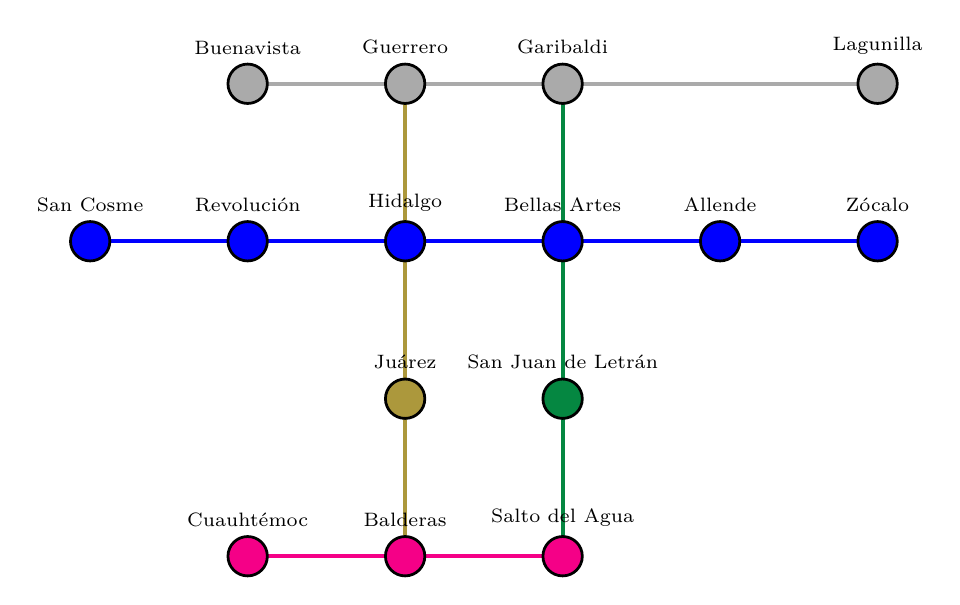
\begin{tikzpicture}
            %Malla 6 x 4
            \Vertex[x=-3,y=3,size=0.5, label=Buenavista,position=above, color=Gris]{A}
            \Vertex[x=-1,y=3,size=0.5, label=Guerrero,position=above, color=Gris]{B}
            \Vertex[x=1,y=3,size=0.5, label=Garibaldi,position=above, color=Gris]{C}
            \Vertex[x=5,y=3,size=0.5, label=Lagunilla,position=above, color=Gris]{D}
            \Edge[color=Gris](A)(B)
            \Edge[color=Gris](B)(C)
            \Edge[color=Gris](C)(D)
            \Vertex[x=-5,y=1,size=0.5, label=San Cosme,position=above, color=Azul]{E}
            \Vertex[x=-3,y=1,size=0.5, label=Revolución,position=above, color=Azul]{F}
            \Vertex[x=-1,y=1,size=0.5, label=Hidalgo,position=above, color=Azul]{G}
            \Vertex[x=1,y=1,size=0.5, label=Bellas Artes,position=above, color=Azul]{H}
            \Vertex[x=3,y=1,size=0.5, label=Allende,position=above, color=Azul]{I}
            \Vertex[x=5,y=1,size=0.5, label=Zócalo,position=above, color=Azul]{J}
            \Edge[color=Azul](E)(F)
            \Edge[color=Azul](F)(G)
            \Edge[color=Azul](G)(H)
            \Edge[color=Azul](H)(I)
            \Edge[color=Azul](I)(J)
            \Edge[color=VerdeOlivo](B)(G)
            \Edge[color=Verde](C)(H)
            \Vertex[x=-1,y=-1,size=0.5, label=Juárez,position=above, color=VerdeOlivo]{K}
            \Vertex[x=1,y=-1,size=0.5, label=San Juan de Letrán,position=above, color=Verde]{L}
            \Edge[color=VerdeOlivo](K)(G)
            \Edge[color=Verde](L)(H)
            \Vertex[x=-3,y=-3,size=0.5, label=Cuauhtémoc,position=above, color=RosaMexicano]{M}
            \Vertex[x=-1,y=-3,size=0.5, label=Balderas,position=above, color=RosaMexicano]{N}
            \Vertex[x=1,y=-3,size=0.5, label=Salto del Agua,position=above, color=RosaMexicano]{O}
            \Edge[color=RosaMexicano](M)(N)
            \Edge[color=RosaMexicano](N)(O)
            \Edge[color=VerdeOlivo](K)(N)
            \Edge[color=Verde](L)(O)
        \end{tikzpicture}
    \end{figure}
    \[
        \left[
            \begin{array}{*{15}c}
                0 & 1 & 0 & 0 & 0 & 0 & 0 & 0 & 0 & 0 & 0 & 0 & 0 & 0 & 0 \\
                1 & 0 & 1 & 0 & 0 & 0 & 1 & 0 & 0 & 0 & 0 & 0 & 0 & 0 & 0 \\
                0 & 1 & 0 & 1 & 0 & 0 & 0 & 1 & 0 & 0 & 0 & 0 & 0 & 0 & 0 \\
                0 & 0 & 1 & 0 & 0 & 0 & 0 & 0 & 0 & 0 & 0 & 0 & 0 & 0 & 0 \\
                0 & 0 & 0 & 0 & 0 & 1 & 0 & 0 & 0 & 0 & 0 & 0 & 0 & 0 & 0 \\
                0 & 0 & 0 & 0 & 1 & 0 & 1 & 0 & 0 & 0 & 0 & 0 & 0 & 0 & 0 \\
                0 & 1 & 0 & 0 & 0 & 1 & 0 & 1 & 0 & 0 & 1 & 0 & 0 & 0 & 0 \\
                0 & 0 & 1 & 0 & 0 & 0 & 1 & 0 & 1 & 0 & 0 & 1 & 0 & 0 & 0 \\
                0 & 0 & 0 & 0 & 0 & 0 & 0 & 1 & 0 & 1 & 0 & 0 & 0 & 0 & 0 \\
                0 & 0 & 0 & 0 & 0 & 0 & 0 & 0 & 1 & 0 & 0 & 0 & 0 & 0 & 0 \\
                0 & 0 & 0 & 0 & 0 & 0 & 1 & 0 & 0 & 0 & 0 & 0 & 0 & 1 & 0 \\
                0 & 0 & 0 & 0 & 0 & 0 & 0 & 1 & 0 & 0 & 0 & 0 & 0 & 0 & 1 \\
                0 & 0 & 0 & 0 & 0 & 0 & 0 & 0 & 0 & 0 & 0 & 0 & 0 & 1 & 0 \\
                0 & 0 & 0 & 0 & 0 & 0 & 0 & 0 & 0 & 0 & 1 & 0 & 1 & 0 & 1 \\
                0 & 0 & 0 & 0 & 0 & 0 & 0 & 0 & 0 & 0 & 0 & 1 & 0 & 1 & 0 \\
            \end{array}
        \right]
    \]
    \newpage
    \section{Grafo y matriz de adyacencia con peso}
    \begin{figure}
        \centering
        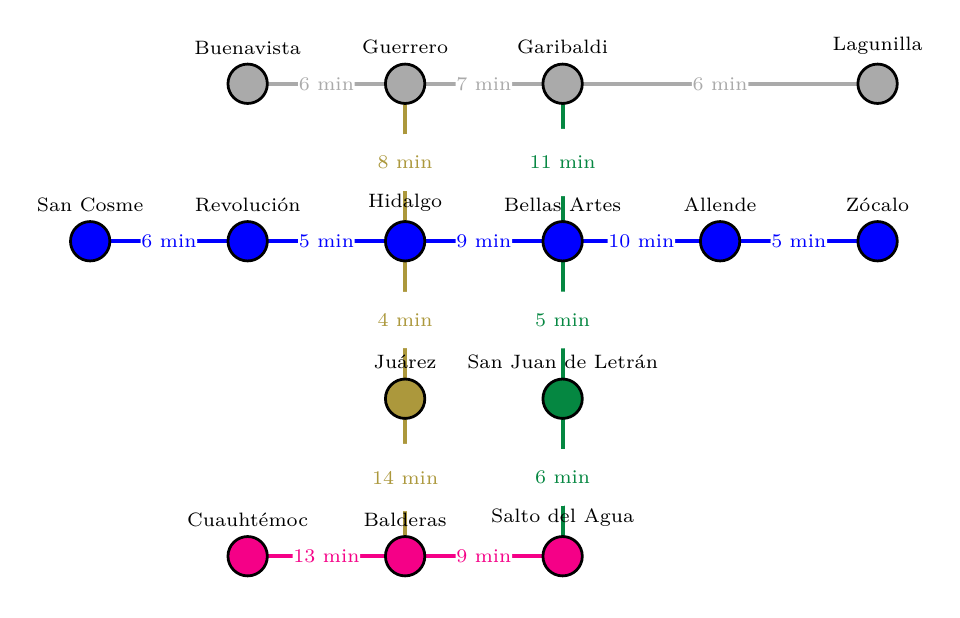
\begin{tikzpicture}
            %Malla 6 x 4
            \Vertex[x=-3,y=3,size=0.5, label=Buenavista,position=above, color=Gris]{A}
            \Vertex[x=-1,y=3,size=0.5, label=Guerrero,position=above, color=Gris]{B}
            \Vertex[x=1,y=3,size=0.5, label=Garibaldi,position=above, color=Gris]{C}
            \Vertex[x=5,y=3,size=0.5, label=Lagunilla,position=above, color=Gris]{D}
            \Edge[color=Gris, label=6 min](A)(B)
            \Edge[color=Gris, label=7 min](B)(C)
            \Edge[color=Gris, label=6 min](C)(D)
            \Vertex[x=-5,y=1,size=0.5, label=San Cosme,position=above, color=Azul]{E}
            \Vertex[x=-3,y=1,size=0.5, label=Revolución,position=above, color=Azul]{F}
            \Vertex[x=-1,y=1,size=0.5, label=Hidalgo,position=above, color=Azul]{G}
            \Vertex[x=1,y=1,size=0.5, label=Bellas Artes,position=above, color=Azul]{H}
            \Vertex[x=3,y=1,size=0.5, label=Allende,position=above, color=Azul]{I}
            \Vertex[x=5,y=1,size=0.5, label=Zócalo,position=above, color=Azul]{J}
            \Edge[color=Azul, label=6 min](E)(F)
            \Edge[color=Azul, label=5 min](F)(G)
            \Edge[color=Azul, label=9 min](G)(H)
            \Edge[color=Azul, label=10 min](H)(I)
            \Edge[color=Azul, label=5 min](I)(J)
            \Edge[color=VerdeOlivo, label=8 min](B)(G)
            \Edge[color=Verde, label=11 min](C)(H)
            \Vertex[x=-1,y=-1,size=0.5, label=Juárez,position=above, color=VerdeOlivo]{K}
            \Vertex[x=1,y=-1,size=0.5, label=San Juan de Letrán,position=above, color=Verde]{L}
            \Edge[color=VerdeOlivo, label=4 min](K)(G)
            \Edge[color=Verde, label=5 min](L)(H)
            \Vertex[x=-3,y=-3,size=0.5, label=Cuauhtémoc,position=above, color=RosaMexicano]{M}
            \Vertex[x=-1,y=-3,size=0.5, label=Balderas,position=above, color=RosaMexicano]{N}
            \Vertex[x=1,y=-3,size=0.5, label=Salto del Agua,position=above, color=RosaMexicano]{O}
            \Edge[color=RosaMexicano, label=13 min](M)(N)
            \Edge[color=RosaMexicano, label=9 min](N)(O)
            \Edge[color=VerdeOlivo, label=14 min](K)(N)
            \Edge[color=Verde, label=6 min](L)(O)
        \end{tikzpicture}
    \end{figure}
    \[
        \left[
            \begin{array}{*{15}c}
                0 & 6 & 0 & 0 & 0 & 0 & 0 & 0 & 0 & 0 & 0 & 0 & 0 & 0 & 0 \\
                6 & 0 & 7 & 0 & 0 & 0 & 8 & 0 & 0 & 0 & 0 & 0 & 0 & 0 & 0 \\
                0 & 7 & 0 & 6 & 0 & 0 & 0 & 11 & 0 & 0 & 0 & 0 & 0 & 0 & 0 \\
                0 & 0 & 6 & 0 & 0 & 0 & 0 & 0 & 0 & 0 & 0 & 0 & 0 & 0 & 0 \\
                0 & 0 & 0 & 0 & 0 & 6 & 0 & 0 & 0 & 0 & 0 & 0 & 0 & 0 & 0 \\
                0 & 0 & 0 & 0 & 6 & 0 & 5 & 0 & 0 & 0 & 0 & 0 & 0 & 0 & 0 \\
                0 & 8 & 0 & 0 & 0 & 5 & 0 & 9 & 0 & 0 & 4 & 0 & 0 & 0 & 0 \\
                0 & 0 & 11 & 0 & 0 & 0 & 9 & 0 & 10 & 0 & 0 & 5 & 0 & 0 & 0 \\
                0 & 0 & 0 & 0 & 0 & 0 & 0 & 10 & 0 & 5 & 0 & 0 & 0 & 0 & 0 \\
                0 & 0 & 0 & 0 & 0 & 0 & 0 & 0 & 5 & 0 & 0 & 0 & 0 & 0 & 0 \\
                0 & 0 & 0 & 0 & 0 & 0 & 4 & 0 & 0 & 0 & 0 & 0 & 0 & 14 & 0 \\
                0 & 0 & 0 & 0 & 0 & 0 & 0 & 5 & 0 & 0 & 0 & 0 & 0 & 0 & 6 \\
                0 & 0 & 0 & 0 & 0 & 0 & 0 & 0 & 0 & 0 & 0 & 0 & 0 & 13 & 0 \\
                0 & 0 & 0 & 0 & 0 & 0 & 0 & 0 & 0 & 0 & 14 & 0 & 13 & 0 & 9 \\
                0 & 0 & 0 & 0 & 0 & 0 & 0 & 0 & 0 & 0 & 0 & 6 & 0 & 9 & 0 \\
            \end{array}
        \right]
    \]

%%%%%%%%%%%%%%%%%%%%%%%%%%%%%%%%%%%%%%%%%%%%%%%%%%%%%%%%%%%%%%%%%%%%%%%%%%%%%%%%%%%%%%%%%%%%%%%%%%%%%%%%%%%%%%%%%%%%%%%%%%%%%%%%%%%%%%%%%%%%%%%

En la siguiente parte del código lo que hacemos es crear una lista de
los vértices a partir de la lista de aristas. Después inicializamos la
matriz \texttt{M}, que será nuestra \textbf{matriz de adyacencia} como
una matriz de ceros.

\begin{Shaded}
\begin{Highlighting}[]
\NormalTok{vertices }\OperatorTok{=}\NormalTok{ []}
\CommentTok{\# Agregamos todos los vértices:}
\ControlFlowTok{for}\NormalTok{ a }\KeywordTok{in}\NormalTok{ aristas:}
\NormalTok{  vertices.append(a[}\DecValTok{0}\NormalTok{])}
\NormalTok{  vertices.append(a[}\DecValTok{1}\NormalTok{])}

\CommentTok{\# Eliminamos los vértices repetidos:}
\NormalTok{vertices }\OperatorTok{=} \BuiltInTok{list}\NormalTok{(}\BuiltInTok{dict}\NormalTok{.fromkeys(vertices))}

\CommentTok{\# Inicializamos la matriz de adyacencia en ceros}
\NormalTok{M }\OperatorTok{=}\NormalTok{[ [}\DecValTok{0} \ControlFlowTok{for}\NormalTok{ v }\KeywordTok{in}\NormalTok{ vertices] }\ControlFlowTok{for}\NormalTok{ v }\KeywordTok{in}\NormalTok{ vertices]}
\end{Highlighting}
\end{Shaded}

\begin{Shaded}
\begin{Highlighting}[]
\NormalTok{vertices}
\end{Highlighting}
\end{Shaded}

\begin{verbatim}
['Buenavista',
 'Guerrero',
 'Garibaldi',
 'Lagunilla',
 'Hidalgo',
 'Bellas Artes',
 'San Cosme',
 'Revolucion',
 'Allende',
 'Zocalo',
 'Juarez',
 'Balderas',
 'San Juan de Letran',
 'Salto del agua',
 'Cuauhtemoc']
\end{verbatim}

\begin{Shaded}
\begin{Highlighting}[]
\NormalTok{M}
\end{Highlighting}
\end{Shaded}

\begin{verbatim}
[[0, 0, 0, 0, 0, 0, 0, 0, 0, 0, 0, 0, 0, 0, 0],
 [0, 0, 0, 0, 0, 0, 0, 0, 0, 0, 0, 0, 0, 0, 0],
 [0, 0, 0, 0, 0, 0, 0, 0, 0, 0, 0, 0, 0, 0, 0],
 [0, 0, 0, 0, 0, 0, 0, 0, 0, 0, 0, 0, 0, 0, 0],
 [0, 0, 0, 0, 0, 0, 0, 0, 0, 0, 0, 0, 0, 0, 0],
 [0, 0, 0, 0, 0, 0, 0, 0, 0, 0, 0, 0, 0, 0, 0],
 [0, 0, 0, 0, 0, 0, 0, 0, 0, 0, 0, 0, 0, 0, 0],
 [0, 0, 0, 0, 0, 0, 0, 0, 0, 0, 0, 0, 0, 0, 0],
 [0, 0, 0, 0, 0, 0, 0, 0, 0, 0, 0, 0, 0, 0, 0],
 [0, 0, 0, 0, 0, 0, 0, 0, 0, 0, 0, 0, 0, 0, 0],
 [0, 0, 0, 0, 0, 0, 0, 0, 0, 0, 0, 0, 0, 0, 0],
 [0, 0, 0, 0, 0, 0, 0, 0, 0, 0, 0, 0, 0, 0, 0],
 [0, 0, 0, 0, 0, 0, 0, 0, 0, 0, 0, 0, 0, 0, 0],
 [0, 0, 0, 0, 0, 0, 0, 0, 0, 0, 0, 0, 0, 0, 0],
 [0, 0, 0, 0, 0, 0, 0, 0, 0, 0, 0, 0, 0, 0, 0]]
\end{verbatim}

Con nuestra matriz \texttt{M} inicializada en ceros y las listas de
aristas y vértices, ahora podemos crear nuestra matriz de adyacencia:

\begin{Shaded}
\begin{Highlighting}[]
\ControlFlowTok{for}\NormalTok{ a }\KeywordTok{in}\NormalTok{ aristas:}
\NormalTok{    i1 }\OperatorTok{=}\NormalTok{ vertices.index(a[}\DecValTok{0}\NormalTok{])}
\NormalTok{    i2 }\OperatorTok{=}\NormalTok{ vertices.index(a[}\DecValTok{1}\NormalTok{])}
\NormalTok{    M[i1][i2] }\OperatorTok{=}\NormalTok{ a[}\DecValTok{2}\NormalTok{]}
\NormalTok{    M[i2][i1] }\OperatorTok{=}\NormalTok{ a[}\DecValTok{2}\NormalTok{]}
\end{Highlighting}
\end{Shaded}

\begin{Shaded}
\begin{Highlighting}[]
\NormalTok{M}
\end{Highlighting}
\end{Shaded}

\begin{verbatim}
[[0, 6, 0, 0, 0, 0, 0, 0, 0, 0, 0, 0, 0, 0, 0],
 [6, 0, 7, 0, 8, 0, 0, 0, 0, 0, 0, 0, 0, 0, 0],
 [0, 7, 0, 6, 0, 11, 0, 0, 0, 0, 0, 0, 0, 0, 0],
 [0, 0, 6, 0, 0, 0, 0, 0, 0, 0, 0, 0, 0, 0, 0],
 [0, 8, 0, 0, 0, 9, 0, 5, 0, 0, 4, 0, 0, 0, 0],
 [0, 0, 11, 0, 9, 0, 0, 0, 10, 0, 0, 0, 5, 0, 0],
 [0, 0, 0, 0, 0, 0, 0, 6, 0, 0, 0, 0, 0, 0, 0],
 [0, 0, 0, 0, 5, 0, 6, 0, 0, 0, 0, 0, 0, 0, 0],
 [0, 0, 0, 0, 0, 10, 0, 0, 0, 5, 0, 0, 0, 0, 0],
 [0, 0, 0, 0, 0, 0, 0, 0, 5, 0, 0, 0, 0, 0, 0],
 [0, 0, 0, 0, 4, 0, 0, 0, 0, 0, 0, 14, 0, 0, 0],
 [0, 0, 0, 0, 0, 0, 0, 0, 0, 0, 14, 0, 0, 9, 13],
 [0, 0, 0, 0, 0, 5, 0, 0, 0, 0, 0, 0, 0, 6, 0],
 [0, 0, 0, 0, 0, 0, 0, 0, 0, 0, 0, 9, 6, 0, 0],
 [0, 0, 0, 0, 0, 0, 0, 0, 0, 0, 0, 13, 0, 0, 0]]
\end{verbatim}

Ahora creamos la función

\texttt{dijktra(idx\_origen,\ idx\_destino)}

que recibe como parámetros:

\begin{itemize}
\item
  \texttt{idx\_origen}: índice del vértice de origen respecto a la lista
  \texttt{aristas}.
\item
  \texttt{idx\_destino}: índice del vértice de destino respecto a la
  lista \texttt{aristas}.
\end{itemize}

Dentro de la función , lo primero que hacemos es crear las listas
\texttt{marcados} y \texttt{no\_marcados} que representan los vértices
ya marcados y los que no respectivamente.

También creamos la lista \texttt{info\_vertices}, que contiene un
diccionario por cada vértice, ese diccionario nos guarda la siguiente
información:

\begin{itemize}
\tightlist
\item
  El nombre del vértice.
\item
  El camino desde el vértice de origen (se inicializa con el propio
  vértice de origen).
\item
  El tiempo (se inicializa con \texttt{sys.maxsize}, nuestro $\infty$).
\end{itemize}

Después agregamos el vértice de origen a marcados y lo quitamos de los
no marcados.

Luego creamos un bucle que se ejecuta mientras el vértice de destino no
se encuentre en la lista de marcados.

Dentro del bucle tomamos el vértice actual como el último de marcados.
Luego vemos en su matriz de adyacencia la información de los vértices
vecinos. Calculamos el tiempo desde el vértice de origen a cada vecino
pasando por el vértice actual y si es menor que el tiempo que ya
correspondía a ese vértice, actualizamos la información.

Después revisamos la información de los vértices no marcados y elegimos
el de menor tiempo para agregarlo a marcados y quitarlo de los no
marcados.

Una vez terminado el bucle, imprimimos el camino más corto.

\begin{Shaded}
\begin{Highlighting}[]
\KeywordTok{def}\NormalTok{ dijkstra(idx\_origen, idx\_destino):}
  
\NormalTok{  marcados }\OperatorTok{=}\NormalTok{ []}
\NormalTok{  no\_marcados }\OperatorTok{=}\NormalTok{ [v }\ControlFlowTok{for}\NormalTok{ v }\KeywordTok{in}\NormalTok{ vertices]}
\NormalTok{  info\_vertices}\OperatorTok{=}\NormalTok{[ \{}\StringTok{"v"}\NormalTok{: v ,}\StringTok{"camino"}\NormalTok{:[vertices[idx\_origen]], }\StringTok{"tiempo"}\NormalTok{:sys.maxsize\} }\ControlFlowTok{for}\NormalTok{ v }\KeywordTok{in}\NormalTok{ vertices]}
  
\NormalTok{  info\_vertices[idx\_origen][}\StringTok{"tiempo"}\NormalTok{] }\OperatorTok{=} \DecValTok{0}
\NormalTok{  marcados.append(vertices[idx\_origen])}
  \KeywordTok{del}\NormalTok{ no\_marcados[vertices.index(marcados[}\OperatorTok{{-}}\DecValTok{1}\NormalTok{])]}

  \ControlFlowTok{while}\NormalTok{ vertices[idx\_destino] }\KeywordTok{not} \KeywordTok{in}\NormalTok{ marcados:}
\NormalTok{    v\_act }\OperatorTok{=}\NormalTok{ marcados[}\OperatorTok{{-}}\DecValTok{1}\NormalTok{]}
\NormalTok{    idx\_act }\OperatorTok{=}\NormalTok{ vertices.index(v\_act)}
  
    \ControlFlowTok{for}\NormalTok{ j }\KeywordTok{in}\NormalTok{ M[idx\_act]:}
      \ControlFlowTok{if}\NormalTok{ j }\OperatorTok{!=} \DecValTok{0}\NormalTok{:}
\NormalTok{        t }\OperatorTok{=}\NormalTok{ info\_vertices[idx\_act][}\StringTok{"tiempo"}\NormalTok{] }\OperatorTok{+}\NormalTok{ j}
\NormalTok{        pos }\OperatorTok{=}\NormalTok{ M[idx\_act].index(j)}
        \ControlFlowTok{if}\NormalTok{ info\_vertices[pos][}\StringTok{"tiempo"}\NormalTok{] }\OperatorTok{\textgreater{}}\NormalTok{ t:}
\NormalTok{          info\_vertices[pos][}\StringTok{"tiempo"}\NormalTok{] }\OperatorTok{=}\NormalTok{ t}
\NormalTok{          info\_vertices[pos][}\StringTok{"camino"}\NormalTok{] }\OperatorTok{=}\NormalTok{ info\_vertices[idx\_act][}\StringTok{"camino"}\NormalTok{].copy()}
\NormalTok{          info\_vertices[pos][}\StringTok{"camino"}\NormalTok{].append(vertices[pos])}

\NormalTok{    minimo }\OperatorTok{=}\NormalTok{ sys.maxsize}

    \ControlFlowTok{for}\NormalTok{ nm }\KeywordTok{in}\NormalTok{ no\_marcados:}
\NormalTok{      idx\_nuevo }\OperatorTok{=}\NormalTok{ vertices.index(nm)}
\NormalTok{      t }\OperatorTok{=}\NormalTok{ info\_vertices[idx\_nuevo][}\StringTok{"tiempo"}\NormalTok{]}
      \ControlFlowTok{if}\NormalTok{ t }\OperatorTok{\textless{}}\NormalTok{ minimo:}
\NormalTok{        minimo }\OperatorTok{=}\NormalTok{ t}
\NormalTok{        v\_act }\OperatorTok{=}\NormalTok{ nm}
\NormalTok{    marcados.append(v\_act)}
\NormalTok{    no\_marcados.remove(v\_act)   }

  \BuiltInTok{print}\NormalTok{(}\SpecialStringTok{f\textquotesingle{}El camino más corto es: }\SpecialCharTok{\{}\NormalTok{info\_vertices[idx\_destino][}\StringTok{"camino"}\NormalTok{]}\SpecialCharTok{\}}\SpecialStringTok{\textquotesingle{}}\NormalTok{)}
\end{Highlighting}
\end{Shaded}

Pedimos al usuario que elija el vértice de origen y el vértice de
destino.

\begin{Shaded}
\begin{Highlighting}[]
\BuiltInTok{print}\NormalTok{(}\StringTok{"Elige el origen:"}\NormalTok{)}
\NormalTok{i }\OperatorTok{=} \DecValTok{0}
\ControlFlowTok{for}\NormalTok{ v }\KeywordTok{in}\NormalTok{ vertices:}
  \BuiltInTok{print}\NormalTok{(}\SpecialStringTok{f"}\SpecialCharTok{\{i\}}\SpecialStringTok{. }\SpecialCharTok{\{v\}}\SpecialStringTok{"}\NormalTok{)}
\NormalTok{  i}\OperatorTok{+=}\DecValTok{1}

\NormalTok{o }\OperatorTok{=} \BuiltInTok{int}\NormalTok{(}\BuiltInTok{input}\NormalTok{())}

\BuiltInTok{print}\NormalTok{(}\StringTok{"Elige el destino:"}\NormalTok{)}
\NormalTok{i }\OperatorTok{=} \DecValTok{0}
\ControlFlowTok{for}\NormalTok{ v }\KeywordTok{in}\NormalTok{ vertices:}
  \BuiltInTok{print}\NormalTok{(}\SpecialStringTok{f"}\SpecialCharTok{\{i\}}\SpecialStringTok{. }\SpecialCharTok{\{v\}}\SpecialStringTok{"}\NormalTok{)}
\NormalTok{  i}\OperatorTok{+=}\DecValTok{1}

\NormalTok{d }\OperatorTok{=} \BuiltInTok{int}\NormalTok{(}\BuiltInTok{input}\NormalTok{())}
\NormalTok{dijkstra(o,d)}
\end{Highlighting}
\end{Shaded}

\begin{verbatim}
Elige el origen:
0. Buenavista
1. Guerrero
2. Garibaldi
3. Lagunilla
4. Hidalgo
5. Bellas Artes
6. San Cosme
7. Revolucion
8. Allende
9. Zocalo
10. Juarez
11. Balderas
12. San Juan de Letran
13. Salto del agua
14. Cuauhtemoc
2
Elige el destino:
0. Buenavista
1. Guerrero
2. Garibaldi
3. Lagunilla
4. Hidalgo
5. Bellas Artes
6. San Cosme
7. Revolucion
8. Allende
9. Zocalo
10. Juarez
11. Balderas
12. San Juan de Letran
13. Salto del agua
14. Cuauhtemoc
14
El camino más corto es: ['Garibaldi', 'Bellas Artes', 'San Juan de Letran', 'Salto del agua', 'Balderas', 'Cuauhtemoc']
\end{verbatim}

\end{document}

